\section{Resultados}
\subsection{Objetivo 1: Algoritmo de trilateración}

Para el cálculo de la posición del usuario se implementó un algoritmo de trilateración en dos dimensiones (x,y), dado que el propósito principal de la aplicación de realidad aumentada es determinar la ubicación del usuario sobre un plano, sin necesidad de considerar su altura exacta en el eje z. En un escenario tridimensional, la trilateración requiere al menos cuatro sensores UWB para resolver la posición completa del usuario. Sin embargo, al limitar el problema al plano bidimensional, fue posible emplear únicamente tres sensores, con la condición de manejar adecuadamente el eje z para evitar que su omisión se tradujera en un error adicional sobre los ejes x e y.

\subsubsection*{Derivación matemática del modelo}

El modelo parte de la ecuación de distancia entre el usuario $(x, y, z)$ y cada sensor $i$:

\[
\sqrt{(x-x_i)^2 + (y-y_i)^2 + (z-z_i)^2} = d_i
\]

Al elevar ambos lados al cuadrado y expandir los términos, se obtiene:

\[
x^2 + y^2 + z^2 - 2x \cdot x_i - 2y \cdot y_i - 2z \cdot z_i + (x_i^2 + y_i^2 + z_i^2) = d_i^2
\]

Para eliminar los términos cuadráticos comunes, se resta una ecuación de referencia (sensor 1) al resto, obteniendo un sistema lineal en las variables $x$, $y$ y $z$:

\[
2x(x_1 - x_i) + 2y(y_1 - y_i) + 2z(z_1 - z_i) = d_i^2 - d_1^2 - x_i^2 - y_i^2 - z_i^2 + x_1^2 + y_1^2 + z_1^2
\]

Cada ecuación puede representarse en la forma general:
\[
A_i x + B_i y + C_i z = D_i
\]
donde los coeficientes son:
\[
A_i = 2(x_1 - x_i), \quad
B_i = 2(y_1 - y_i), \quad
C_i = 2(z_1 - z_i), \quad
D_i = d_i^2 - d_1^2 - x_i^2 - y_i^2 - z_i^2 + x_1^2 + y_1^2 + z_1^2
\]

De esta manera, para $n$ sensores se obtienen $n-1$ ecuaciones lineales que pueden expresarse matricialmente como:


\[
\begin{bmatrix}
A_{1x} & A_{1y} & A_{1z}\\
A_{2x} & A_{2y} & A_{2z} \\
\vdots & \vdots & \vdots \\
A_{n-1x} & A_{n-1y} & A_{n-1z}
\end{bmatrix}
\begin{bmatrix}
x \\ y \\ z
\end{bmatrix}
=
\begin{bmatrix}
A_{1d} \\ A_{2d} \\ \vdots \\ A_{n-1d}
\end{bmatrix}
\]


Dado que el interés del sistema se centra en la ubicación sobre el plano horizontal, se asumió que todos los sensores se encuentran a una misma altura ($z_i = z_1$), simplificando el sistema a dos dimensiones. Esta simplificación elimina el término asociado a $z$ y reduce el problema a la intersección de tres circunferencias en el plano $(x, y)$.

El sistema puede producir dos posibles soluciones para la coordenada $z$ cuando las circunferencias se intersectan, o bien soluciones imaginarias cuando no existe intersección exacta. Dado que la coordenada $z$ no es relevante para la aplicación, se adoptó la siguiente estrategia:
\begin{itemize}
  \item Si el discriminante era positivo, se resolvía completamente el sistema y se tomaba la solución con $z$ positiva.
  \item Si el discriminante era negativo, se fijaba el valor de $z = 0$.
\end{itemize}

Este procedimiento permitió compensar parcialmente el efecto de la elevación en las mediciones, evitando que el error en la componente vertical se propagara hacia las coordenadas de interés. Para reforzar esta estrategia, se colocaron todos los sensores a una misma altura, de manera que la coordenada $z$ asignada a cada beacon fuera arbitraria pero consistente en todo el sistema.

\subsubsection*{Implementación del algoritmo en Swift}

El algoritmo fue implementado en el lenguaje \texttt{Swift} como parte del plugin nativo de localización para iOS. La función principal, \texttt{do\_trilateration}, recibe como entrada un conjunto dinámico de sensores activos, y selecciona automáticamente las tres anclas más recientes basándose en su marca de tiempo (\textit{timestamp}). Esta estrategia de selección garantiza que las mediciones correspondan a señales coherentes temporalmente, evitando inconsistencias en el cálculo espacial.

Cada ancla contiene su posición $(x_i, y_i, z_i)$ y la distancia medida $d_i$. Estos datos se utilizan para construir las ecuaciones linealizadas y resolver el sistema mediante una formulación explícita derivada de las expresiones anteriores.

La función \texttt{trilaterate\_3D} implementa la resolución directa del sistema para tres anclas, utilizando la ancla 1 como referencia. El algoritmo obtiene las constantes intermedias $A$, $B$, $C$, $D$, $E$, $F$, $G$, $H$ correspondientes a las dos ecuaciones independientes, y a partir de ellas se construye un sistema auxiliar para despejar el eje $z$:

\[
\begin{cases}
A x + B y + C z = D \\
E x + F y + G z = H
\end{cases}
\]

De este sistema se derivan las relaciones:
\[
z = \frac{-B G + C F}{A F - E B}x + \frac{-B H + D F}{A F - E B}, \quad
y = \frac{A G - E C}{A F - E B}x + \frac{A H - E D}{A F - E B}
\]

Sustituyendo en la ecuación del primer sensor se obtiene una ecuación cuadrática en $z$, evaluando el discriminante $\Delta = b^2 - 4ac$:
\begin{itemize}
    \item Si $\Delta > 0$, el sistema devuelve la primera raíz real para $z$.
    \item Si $\Delta < 0$, se asigna $z=0$, evitando la propagación de errores al plano horizontal.
\end{itemize}

\subsubsection*{Extensión a multilateración y resolución mediante ecuaciones normales}

Si bien el modelo de trilateración permitió determinar la posición en dos dimensiones utilizando tres sensores, su desempeño dependía fuertemente de la precisión de las mediciones individuales. Para mitigar el impacto del ruido y mejorar la estabilidad del posicionamiento, se implementó una extensión del modelo basada en multilateración, que permite aprovechar simultáneamente más de tres sensores (hasta seis en las pruebas realizadas).

En este caso, el sistema se expresa de forma general como:

\[
\begin{bmatrix}
A_{1x} & A_{1y} & A_{1z}\\
A_{2x} & A_{2y} & A_{2z}\\
\vdots & \vdots & \vdots\\
A_{n-1x} & A_{n-1y} & A_{n-1z}
\end{bmatrix}
\begin{bmatrix}
x \\ y \\ z
\end{bmatrix}
=
\begin{bmatrix}
A_{1d}\\
A_{2d}\\
\vdots\\
A_{n-1d}
\end{bmatrix}
\]

que puede escribirse compactamente como:

\[
A \mathbf{x} = \mathbf{b}
\]

Cuando el número de sensores $n$ es mayor a tres, el sistema se vuelve sobredeterminado —es decir, no existe un único vector $\mathbf{x}$ que satisfaga exactamente todas las ecuaciones simultáneamente debido a errores de medición y ruido. En este escenario, la estrategia consiste en encontrar la mejor aproximación en el sentido de los mínimos cuadrados, lo cual se consigue resolviendo la ecuación normal asociada:

\[
A^T A \mathbf{x} = A^T \mathbf{b}
\]

\paragraph{Derivación de la ecuación normal}

Sea el sistema $A\mathbf{x} = \mathbf{b}$ con $A \in \mathbb{R}^{m \times n}$ y $m > n$. Dado que el sistema es inconsistente, $\mathbf{b}$ no pertenece al espacio columna de $A$ ($\mathbf{b} \notin \text{col}(A)$). Sin embargo, existe un vector $\hat{\mathbf{x}}$ tal que $A\hat{\mathbf{x}}$ representa la proyección ortogonal de $\mathbf{b}$ sobre $\text{col}(A)$, minimizando el error cuadrático:

\[
A\hat{\mathbf{x}} = \text{proj}_{\text{col}(A)}(\mathbf{b})
\]

\[
\mathbf{b} - A\hat{\mathbf{x}} = \mathbf{b} - \text{proj}_{\text{col}(A)}(\mathbf{b})
\]

Multiplicando ambos lados por $A^T$ se obtiene:

\[
A^T(\mathbf{b} - A\hat{\mathbf{x}}) = 0
\]

\[
A^TA\hat{\mathbf{x}} = A^T\mathbf{b}
\]

Esta formulación corresponde al sistema de ecuaciones normales, cuya solución $\hat{\mathbf{x}}$ representa el punto que minimiza la suma de los errores al cuadrado entre las distancias medidas y las distancias modeladas. Geométricamente, esto equivale a proyectar el vector $\mathbf{b}$ sobre el subespacio generado por las columnas de $A$, como se muestra en la Figura~\ref{fig:projection}.

\tdplotsetmaincoords{70}{110}
\begin{tikzpicture}[tdplot_main_coords, scale=2]

% Define the plane (column space)
\filldraw[green!20, opacity=0.6] 
    (0,0,0) -- (2,0,0) -- (2,2,0.5) -- (0,2,0.5) -- cycle;

% Draw axes
\draw[->, thick] (0,0,0) -- (2.5,0,0) node[below] {$x$};
\draw[->, thick] (0,0,0) -- (0,2.5,0) node[right] {$y$};
\draw[->, thick] (0,0,0) -- (0,0,2.5) node[above] {$z$};

% Define points
\coordinate (O) at (0,0,0);
\coordinate (b) at (1.5,1.5,2);  % Original vector
\coordinate (proj) at (1.5,1.5,0.375); % Projection onto plane

% Draw projection line (dashed)
\draw[dashed, gray, thick] (b) -- (proj);

% Draw vectors
\draw[->, very thick, red] (O) -- (b) node[above right] {$\mathbf{b}$};
\draw[->, very thick, blue] (O) -- (proj) node[below left] {$\text{proj}_{\text{Col}(A)}\mathbf{b}$};

% Draw error vector (perpendicular component)
\draw[->, thick, orange] (proj) -- (b) node[midway, right] {$\mathbf{e}$};

% Label the plane - moved to back corner
\node[green] at (0.3, 1.8, 0.4) {$\text{Col}(A)$};

% Optional: draw right angle indicator
\draw[thick] (proj) -- ++(0.2,0,0) -- ++(0,0,0.2) -- ++(-0.2,0,0);

\end{tikzpicture}

% \begin{figure}[H]
%     \centering
%     \includegraphics[width=0.6\textwidth]{images/projection.png}
%     \caption{Proyección del vector $\mathbf{b}$ sobre el espacio columna de $A$, base conceptual de las ecuaciones normales.}
%     \label{fig:projection}
% \end{figure}

\paragraph{Implementación en Swift}

La multilateración se implementó mediante la función \texttt{multilateration()}, que construye las matrices del sistema y aplica las ecuaciones normales para resolver el vector de posición en tiempo real. El proceso se ejecuta en tres etapas:

\begin{enumerate}
    \item \textbf{Construcción de matrices:} La función \texttt{multInitializeMatrixVector()} genera la matriz $A$ y el vector $\mathbf{b}$ en base a las posiciones y distancias de cada ancla, tomando una de ellas como referencia o \textit{pivot}.
    \item \textbf{Cálculo de las ecuaciones normales:} Se obtiene el producto $A^TA$ y $A^T\mathbf{b}$ mediante multiplicación matricial, creando un sistema cuadrado de dimensión $3 \times 3$.
    \item \textbf{Resolución del sistema:} El sistema resultante se resuelve mediante el método de Gauss-Jordan, devolviendo el vector de posición $(x, y)$.
\end{enumerate}

\begin{lstlisting}[language=Swift, caption={Implementación del método de multilateración en Swift.}]
private func multilateration(anchors: [Anchor]) -> Vector2D {
    let (matrix, vector) = multInitializeMatrixVector(anchors: anchors)
    let n = matrix.count / 3
    let transposedMatrix = transpose(matrix: matrix, rows: n , cols: 3)
    
    let lhs = matrixMultiplication(A: transposedMatrix, rowsOfA: 3,
                                   B: matrix, colsOfB: 3, sharedDim: n)
    let rhs = matrixMultiplication(A: transposedMatrix, rowsOfA: 3,
                                   B: vector, colsOfB: 1, sharedDim: n)
    
    let result = gaussJordan(A: lhs, n: 3, b: rhs)
    return Vector2D(x: result[0], y: result[1])
}
\end{lstlisting}

Esta formulación basada en ecuaciones normales proporciona una estimación más robusta de la posición, al reducir la sensibilidad del sistema frente a errores individuales en las mediciones de distancia. En las pruebas experimentales, la multilateración permitió estabilizar significativamente el cálculo de posición respecto al modelo de trilateración pura, generando trayectorias más suaves y coherentes con el movimiento real del usuario.


\subsubsection*{Validación experimental y observaciones}

Una vez implementado el algoritmo de trilateración en 2D, se realizaron pruebas controladas con tres sensores Estimote UWB para evaluar su funcionamiento. La primera prueba se llevó a cabo en un salón del campus universitario, con el objetivo de obtener una visualización inicial del posicionamiento calculado. En esta etapa se generó una animación (GIF) que mostraba en tiempo real la estimación de la ubicación del usuario.

En dichas pruebas preliminares se observó que las posiciones estimadas presentaban una variabilidad considerable, aun cuando el dispositivo se mantenía estático. Esta fluctuación —visible como movimientos erráticos del punto de localización en la animación— evidenció la presencia de ruido significativo en las mediciones de distancia obtenidas de los sensores.

Posteriormente, se realizó una segunda fase de pruebas en un entorno controlado, específicamente en un cuarto rectangular donde los sensores se dispusieron a una misma altura y en posiciones fijas previamente medidas. En este escenario se registraron las coordenadas calculadas por la trilateración a lo largo del tiempo, mientras el usuario se desplazaba en diagonal entre el origen y el primer cuadrante del plano de referencia.

\begin{figure}[H]
    \centering
    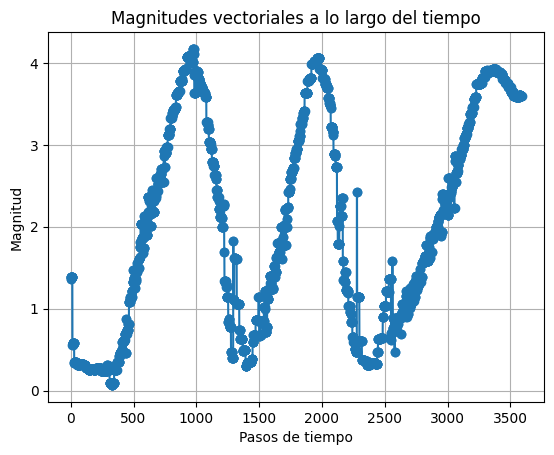
\includegraphics[width=0.8\textwidth]{images/jitter.png}
    \caption{Gráfica de la magnitud del vector de posición a lo largo del tiempo, mostrando el jitter observado durante la trilateración 2D.}
    \label{fig:jitter}
\end{figure}

Para analizar cuantitativamente las variaciones de posición, se calculó la magnitud del vector de posición $ \sqrt{x^2 + y^2} $ y se graficó su evolución temporal. Dado que el movimiento real seguía una trayectoria diagonal y uniforme, se esperaba que la magnitud de la posición oscilara entre 0 y un valor máximo positivo, describiendo un patrón aproximadamente sinusoidal a lo largo del tiempo. Sin embargo, la gráfica resultante (Figura~\ref{fig:jitter}) mostró oscilaciones abruptas e irregulares superpuestas a esta tendencia esperada, confirmando la presencia de jitter y ruido de alta frecuencia en las estimaciones de posición.

Estos resultados demostraron que, aunque la trilateración permitía calcular posiciones válidas en el plano x,y, la señal obtenida era altamente inestable y no adecuada para su uso directo en una aplicación de realidad aumentada sin aplicar técnicas adicionales de filtrado o suavizado.
